\documentclass[12pt]{article}
\usepackage{preamble}

\pagestyle{fancy}
\fancyhead[LO,LE]{Физические основы компьютерных \\ и сетевых технологий}
\fancyhead[RO,RE]{Лекции Музыченко Я. Б.}

\fancyfoot[L]{\scriptsize исходники найдутся тут: \\ \url{https://github.com/pelmesh619/itmo_conspects} \Cat}

\renewcommand{\thesection}{}

\begin{document}

    \tableofcontents
    \clearpage

        % begin physics1_2024_09_02.tex

    \section{0. Вводная лекция}

    Задается вопрос: зачем обучающимся программистам нужна физика в учебном плане?

    Приводятся цитаты Л. Богуславского, одного из крупнейших IT инвесторов, и Б. Страуструпа, которые считают,
    что такие фундаментальные дисциплины, как математика, физика, иностранный язык, способствуют развитию
    мышления человека

    Такие компании, как Bell Labs и IBM создали прорывные изобретения в области физики, на основе которых
    построены компьютерные технологии

    В 3-ем семестре курс физики будет состоять из классической механики и основ электричества

    В 4-ом семестре будут темы магнетизма, колебаний, волн и волновых процессов

    В 5-ом семестре будут рассматриваться оптика, основы квантовой физики и квантовые вычисления

    Занятия состоят из лекций, практических и лабораторных занятий.
    Всего в 3-ем семестре будут 5 лабораторных работ


    \section{1. Современная физическая картина мира. Кинематика материальной точки}

        \begin{tcolorbox}[colframe=blue!25, colback=blue!10, title=\textbf{План лекции}]

        \footnotesize
        \begin{itemize}
            \item Историческая справка
            \item Методы и модели в физике
            \item Изучаемые объекты
            \item Физика и другие науки
            \item Фундаментальные взаимодействия
            \item Кинематика материальной точки. Начало
        \end{itemize}
    \end{tcolorbox}



    \textbf{Физика} - раздел естествознания, изучающий свойства и формы движения материи.
    Под материей понимают вещество и поля.

    Научный метод: сначала проводятся наблюдения и эксперименты, из которых выдвигается гипотеза и ищется
    адекватная математическая модель, эта гипотеза проверяется, и если она подтверждается,
    то формируется \textit{теория}

    Пример - открытие Нептуна: в 1781-1845 годах наблюдались аномалии в движении Урана, в 1845 проведение расчетов
    координат новой планеты, а в 1846 обнаружилась новая планета

    Принцип соответствия (Н. Бор, 1923 г.) - каждая новая теория должна включать предыдущую как частный случай

    Изучаемые объекты: вселенная, галактики, звездные системы и планеты, экосистемы, макротела, молекулы, атомы, ядра,
    элементарные частицы

    Всего в физике существуют 4 фундаментальных взаимодействия:

    \begin{tabular}{c|c|c}
        Взаимодействие   & Квант поля & Область взаимодействия                        \\ \hline
        Гравитационное   & гравитон   & масса                                         \\
        Электромагнитное & фотон      & все заряженные частицы, атомы, электротехника \\
        Слабое           & бозон      & радиоактивный распад                          \\
        Сильное          & глюон      & атомные ядра, фундаментальные частицы         \\
    \end{tabular}

    Механика - раздел физики, изучающий механическое движение, то есть движение тел в пространстве и времени.
    Механическое движение тел ОТНОСИТЕЛЬНО.

    \begin{tabular}{c|c|c|}
        & $\ll 3 \cdot 10^8$ м/с & $\approx 3 \cdot 10^8$ м/с \\ \hline
        $\gg 1$ нм & Классическая           & Релятивистская             \\ \hline
        $\ll 1$ нм & Квантовая              & Квантовая теория поля      \\ \hline
    \end{tabular}

    Материальная точка - тело, размерами которого можно пренебречь в условиях данной задачи

    Абсолютно твердое тело (АТТ) - система материальных точек, расстояние между которыми не меняется
    в процессе движения (деформации в процессе движения пренебрежимо малы)

    Тело отсчета - тело, относительно которого определяется положение других тел в пространстве

    Система отсчета - совокупность тела отсчета, связанной с ним системы координат и синхронизированных между собой часов

    % векторный, координатный и естественный способы

    Степени свободы - число независимых скалярных величин, однозначно определяющих положение тела в пространстве

    Материальная точка: $3$ степени свободы

    Система N материальных точек: $3N$ степени свободы

    АТТ: $6$ степеней свободы

    Система единиц (\deutscht{le System International d'unites}), 1960

    $[t] = $ с \quad $[S, l] = $ м

    7 основных единиц:

    $[S] = $ м \quad $[T] = $ К

    $[m] = $ кг \quad $[\nu] = $ моль

    $[t] = $ с \quad $[l] = $ Кд

    $[q] = $ Кл

    Изначально все физические единицы основывались на материальных предметов, из-за которых точности единиц была низкой,
    но недавно все единицы были переопределены на основе физических констант.

    В природе нет абсолютно точных вычислений. Измерение любой физической величины без погрешности не имеет смысла!
    % end physics1_2024_09_02.tex

    % begin physics1_2024_09_09.tex

    \section{2. Кинематика материальной точки}

    \begin{tcolorbox}[colframe=blue!25, colback=blue!10, title=\textbf{План лекции}]

        \footnotesize
        \begin{itemize}
            \item Основные способы описания движения

            \item Основные понятия кинематики

            \item Кинематика поступательного и вращательного движения

            \item Прямая и обратная задачи кинематики

            \item Численные методы при решении задач
        \end{itemize}
    \end{tcolorbox}

    \Def Кинематика - раздел механики, изучающий движение тел, независимо от причин, вызывающих это движение.

    \Def Траектория - линия, по которой движется материальная точка в пространстве

    \Def Путь - длина траектории

    \Def Перемещение - вектор, проведенный из начальной точки в конечную

    \smallvspace

    \textbf{Способы описания движения}

    \begin{multicols}{3}

        \begin{tcolorbox}
            Векторный способ
        \end{tcolorbox}

        \begin{tcolorbox}
            Координатный способ
        \end{tcolorbox}

        \begin{tcolorbox}
            Естественный (траекторный) способ
        \end{tcolorbox}

    \end{multicols}

    \begin{multicols}{3}

        Положение точки может быть однозначно определено с помощью радиус-вектора

        \smallvspace

        Положение точки может быть однозначно определено с помощью трех скалярных координат

        Положение точки определяется дуговой координатой

        \phantom{.}

    \end{multicols}

    \textbf{Векторный способ}

    $\vec{r_1}, \vec{r_2}$ - радиус-векторы, определяющие положения материальной точки в 1 и 2

    $\Delta \vec{r} = \vec{r_2} - \vec{r_1}$ - перемещение материальной точки

    \Def Скорость - векторная физическая величина, характеризующая быстроту перемещения материальной точки

    Средняя скорость - $\Pair{\vec{v}} = \frac{\Delta \vec{r}}{\Delta t}$

    Мгновенная скорость - $\vec{v} = \lim_{\Delta t \to 0} \frac{\Delta \vec{r}}{\Delta t} = \frac{d \vec{r}}{dt}$

    Средняя путевая скорость - $v_{\text{ср}} = \frac{\Delta S}{\Delta t}$

    \Def Ускорение - векторная физическая величина, характеризующая быстроту изменения скорости материальной точки

    Среднее ускорение - $\Pair{\vec{a}} = \frac{\Delta \vec{v}}{\Delta t}$

    Мгновенное ускорение - $\vec{a} = \lim_{\Delta t \to 0} \frac{\Delta \vec{v}}{\Delta t} = \frac{d \vec{v}}{dt}$

    % годограф скорости

    \textbf{Координатный способ}

    В координатном способе положение точки описано 3 координатами $x, y, z$ (в данном случае в ДПСК)

    $|r| = \sqrt{x^2 + y^2 + z^2}$

    $\vec{r} (t) = r_x (t) \vec{\imath} + r_y (t) \vec{\jmath} + r_z (t) \vec{k} = x(t) \vec{\imath} + y(t) \vec{\jmath} + z(t) \vec{k}$

    $\vec{v} (t) = \frac{d \vec{r}}{dt} = \frac{dx}{dt} \vec{\imath} + \frac{dy}{dt} \vec{\jmath} + \frac{dz}{dt} \vec{k}$

    $\vec{v} (t) = v_x(t)\vec{\imath} + v_y(t) \vec{\jmath} + v_z(t) \vec{k}$

    $|\vec{v}| = \sqrt{v_x^2 + v_y^2 + v_z^2}$


    % ускорение

    Прямая задача:

    $\vec{r}(t), x(t), y(t), z(t) \longrightarrow \vec{v}(t), \vec{a}(t), v_x, v_y, v_z, a_x, a_y, a_z$

    Решением является дифференцирование

    Обратная задача:

    $\vec{a}(t), a_x, a_y, a_z \longrightarrow \vec{v}(t), \vec{r}(t), x(t), y(t), z(t)$

    Для обратной задачи решением является интегрирование

    $\vec{v} = \frac{d\vec{r}}{dt} \quad d\vec{r} = \vec{v}dt \quad \Delta\vec{r} = \int_{t_1}^{t_2} \vec{v}dt$

    \begin{tcolorbox}
        $\vec{r} = \vec{r_0} + \Delta \vec{r} = \vec{r_0} + \int_{t_1}^{t_2} \vec{v}dt$
    \end{tcolorbox}

    Аналогично для ускорения

    Численное решение ОДУ (обыкновенного дифференциального уравнения) $\frac{dy}{dx} = f(x, y)$ на отрезке $[x_0, x_n]$ при условии $y(x_0) = y_0$

    Разбиваем отрезок $[x_0, x_n]$ на конечное число частей введением узловых точек

    Шаг разбиения: $h = \frac{x_N - x_0}{N}$

    По определению производной $\frac{dy}{dx} = \frac{y_{i + 1} - y_i}{h}$, из этого:

    \begin{tcolorbox}
        Формула Эйлера: $y_{i + 1} = y_i + hf(x_i, y_i)$
    \end{tcolorbox}

    $dy = f(x, y) dx$

    $\Delta y = y_{i + 1} - y_i = \int_{x_i}^{x_{i + 1}} f(x, y) dx$

    \textbf{Естественный (траекторный) способ}

    Если траектория точки заранее известна, то положение точки задается дуговой координатой $l(t)$

    $\vec{v} = v_\tau \vec{\tau} \quad v_\tau \frac{dl}{dt} |\vec{\tau}| = 1$

    $\vec{a} = \frac{d\vec{v}}{dt} = \frac{dv_\tau}{dt} \vec{\tau} + \frac{d\vec{\tau}}{dt} v_\tau \quad\quad\quad \frac{d\tau}{dt} = \frac{d\tau}{dl} \cdot \frac{dl}{dt} = \frac{d\tau}{dl} v_\tau$

    $\vec{a} = \frac{d\vec{v}}{dt} = \frac{dv_\tau}{dt} \vec{\tau} + \frac{d\vec{\tau}}{dt} v_\tau^2 $

    $d\tau = \tau d\alpha$

    $dl = R d\alpha \quad\quad\quad d\vec{\tau} \uparrow\uparrow \vec{n}$

    $R$ - радиус кривизны траектории

    $\vec{\alpha} = \frac{dv_\tau}{dt} \vec{\tau} + \frac{1}{R} v_\tau^2 \vec{n} \quad\quad\quad \vec{a} = \vec{a_\tau} + \vec{a_n}$

    Тангенциальное ускорение отвечает за изменение модуля скорости, направлено по касательной к траектории движения

    Нормальное ускорение отвечает за изменение направления вектора скорости, направлено к центру кривизны траектории
    % end physics1_2024_09_09.tex

    % begin physics1_2024_09_16.tex

    \section{3.
    Кинематика вращательного движения.
    Динамика материальной точки}

    \begin{tcolorbox}[colframe=blue!25, colback=blue!10, title=\textbf{План лекции}]

        \footnotesize
        \begin{itemize}
            \item Угловые величины: угол поворота, угловая скорость

            \item Взаимосвязь между линейными и угловыми величинами

            \item Плоское движение

            \item Динамика материальной точки

            \item Законы Ньютона. Силы в механике

            \item Принципы работы акселерометра
        \end{itemize}
    \end{tcolorbox}

    \subsection{Движение по окружности}

    Возьмем точку $A$, положение которое определим через $\vec{r}$. Точка $A$ движется по окружности вокруг неподвижной оси $OO^\prime$

    Тогда $d\vec{r}$ - перемещение, $d\vec{\varphi}$ - элементарный угол поворота (вектор определяет в какую сторону, по часовой или против,
    обращается по окружности тело; вектор направлен перпендикулярно окружности)

    $|d\vec{r}| = Rd\varphi = r \cdot \sin \alpha d \varphi$

    $R = r \cdot \sin \alpha$

    $d\vec{r} = [d \vec{\varphi} \vec{r}]$ \hfill {\scriptsize здесь и далее $[\vec{x}\vec{y}]$ - векторное произведение}

    Угловая скорость - векторная величина, показывающая как меняется угол поворота тела со временем: $\Pair{\omega} = \frac{\Delta \varphi}{\Delta t} \quad\quad\quad \vec{\omega} = \frac{d\vec{\varphi}}{dt}$

    Направление совпадает с направлением угла поворота $d\vec{\varphi}$: $\vec{\omega} \uparrow\uparrow d\vec{\varphi}$

    Угловое ускорение - векторная величина, показывающая как меняется угловая скорость тела со временем

    $\Pair{\beta} = \frac{\Delta \omega}{\Delta t} \quad\quad \vec{\beta} = \frac{d\vec{\omega}}{dt} = \frac{d^2 \vec{\varphi}}{dt^2}$

    Направление совпадает с направлением вектора изменения скорости $\Delta \vec{\omega}$: $\vec{\beta} \uparrow\uparrow d\vec{\omega}$

    $d\vec{r} = [d\vec{\varphi} \vec{r}]$

    $dr = d\varphi \cdot r \cdot \sin \alpha = d\varphi \cdot R$

    Выразим скорость $\vec{v} = \frac{d\vec{r}}{dt} = [\frac{d\vec{\varphi}}{dt}\vec{r}] = [\vec{\omega} \vec{r}]$

    $v = \omega \cdot r \cdot \sin \alpha = \omega \cdot R$

    Выразим ускорение: $\vec{a} = \frac{d\vec{v}}{dt} = [\frac{d\vec{\omega}}{dt} \vec{r}] + [\vec{\omega} \frac{d\vec{r}}{dt}] = [\vec{\beta}\vec{r}] + [\vec{\omega}\vec{v}] = \vec{a}_\tau + \vec{a}_n$

    $\vec{a}_\tau$ называют тангенциальным ускорением (напраленным по касательной), $\vec{a}_n$ - нормальным (направленным к центру)

    $a_\tau = \beta \cdot r \cdot \sin\alpha = \beta \cdot R$

    Перемещение, путь, скорость:

    \begin{multicols}{2}

        $d\vec{r} = [d\vec{\varphi} \vec{\rho}] (\vec{\rho}\text{ - вектор радиуса окружности})$

        $dr = d\varphi \cdot R$

        $S = \varphi \cdot R$

        $\vec{v} = [\vec{\omega} \vec{\rho}]$

        $v = \omega \cdot R$

    \end{multicols}

    Ускорение: $\vec{a} = [\vec{\beta}\vec{r}] + [\vec{\omega}\vec{v}]$

    \begin{multicols}{3}

        $\vec{a}_\tau = [\vec{\beta}\vec{r}]$

        $a_\tau = \beta \cdot R$

        $\vec{a}_n = [\vec{\omega}\vec{v}] = [\vec{\omega}[\vec{\omega}\vec{\rho}]]$

        $a_n = \omega^2 R = \frac{1}{R} v^2$

        $T = \frac{2\pi}{\omega} = \frac{1}{\nu}$ - период

        $\nu = \frac{\omega}{2\pi} = \frac{1}{T}$ - частота

    \end{multicols}

    Плоское движение - движение твердого тела, при котором каждая его точка движется в плоскости,
    параллельной некоторой неподвижной в данной системе отсчета плоскости

    $\vec{r} = \vec{r}_0 + \vec{r}^\prime$

    $d\vec{r} = d\vec{r}_0 + d\vec{r}^\prime = d\vec{r}_0 + [d\vec{\varphi}\vec{r}]$

    $\vec{v} = \vec{v}_0 + [\vec{\omega}\vec{r}]$

    $\vec{v}_C$ - скорость центра колеса относительно точки отсчета

    $\vec{v}_{\text{вр}}$ - скорость точек колеса относительное его центра

    \Def Динамика - раздел механики, изучающий причины, вызывающие движение тел

    1687 г. - законы Ньютона, основа классической механики (механики Ньютона), обобщение большего количества опытов (Г. Галилей)

    Классическая механика - частный случай  1) СТО при скоростях много меньших скорости света $v \ll c$;
    2) квантовой механики при массах, много больших массы атома

    В динамике существуют различия между системами отсчета и преимущества одних СО над другими.

    Существуют такие системы отсчета, относительно которых свободное тело (тело, на которое не действуют другие тела) движется равномерно
    и прямолинейно или находится в состоянии покоя. Таким системы называются инерциальными (ИСО)

%    Земля $a_n = 3.4 \frac{\text{см}}{\text{с}^2}$
%
%    Центр Земли $a_n = 0.6 \frac{\text{см}}{\text{с}^2}$
%
%    Земля $a_n = 3 \cdot 10^{-8} \frac{\text{см}}{\text{с}^2}$
    % for later use i think

    \mediumvspace

    \textbf{Принцип относительности Галилея:}

    Любая СО, движущаяся с постоянной скоростью относительно ИСО, также является ИСО. Тогда справедливо любое из этих утверждений:

    \begin{enumerate}
        \item все ИСО эквивалентны друг другу по своим механическим свойствам
        \item во всех ИСО свойства пространства и времени одинаковы
        \item законы механики одинаковы во всех ИСО
    \end{enumerate}

    % сложное движение земли
    % перечитываю это и не понимаю, че было

    Преобразования Галилея - преобразования координат при переходе от одной ИСО к другой

    $K, K^\prime$ - ИСО

    $\vec{V}$ - скорость, с которой движется СО $K^\prime$ относительно $K$
    $t = t^\prime$

    $\vec{r} = \vec{r}^\prime + \vec{V}t$

    $\vec{c} = \vec{v}^\prime + \vec{V}$

    $\vec{a} = \vec{a}^\prime$

    \Def Сила - физическая величина, определяющая количественную характеристику и напраление воздействия, оказываемого на данное тело
    со стороны других тел.

    Силы условно можно разделить на силы, возникающие при непосредственном контакте (силы трения, давления) и на силы,
    возникающие через поля (электрические, гравитационные).

    \Def Инертная масса - мера инертности тела, то есть способности тела сохранять свою скорость при движении

    \Def Гравитационная масса - мера гравитацонного взаимодействия, величина, определяющая вес тел.

    $m_{\text{ин}} = m_{\text{гр}}$ с точностью до $10^{-13}$ кг

    В классической механике 1) масса - величина аддитивная ($m_1 + m_2 + \dots = m$); 2) $m = const$


    \subsection{Законы Ньютона}


    \begin{tcolorbox}[colframe=green!25, colback=green!10, title=\textbf{I закон Ньютона}, coltitle=black]
        Существуют такие системы отсчёта, называемые инерциальными, относительно которых материальные точки, когда на них не действуют никакие силы (или действуют силы взаимно уравновешенные), находятся в состоянии покоя или равномерного прямолинейного движения.
    \end{tcolorbox}


    \begin{tcolorbox}[colframe=green!25, colback=green!10, title=\textbf{II закон Ньютона}, coltitle=black]
        Ускорение тела пропорционально действующей на него силе и обратно пропорционально его массе $\vec{a} = \frac{\vec{F}}{m}$
    \end{tcolorbox}

    Под равнодействующей всех сил понимают векторную сумму всех сил, действующих на тело (принцип суперпозиции)

    $\vec{F} = \frac{d\vec{p}}{dt}$ - II закон в импульсной (дифференциальной) форме

    \begin{tcolorbox}[colframe=green!25, colback=green!10, title=\textbf{III закон Ньютона}, coltitle=black]
        Силы, с которыми два тела действуют друг на друга равны по модулю и направлены в противоположные стороны $\vec{F}_{12} = -\vec{F}_{21}$
    \end{tcolorbox}

    Закон Гука: $F = k|\Delta l|$ - сила упругости пропорциональна изменению длины тела

    Акселерометр - прибор, измеряющий ускорение, точнее проекцию кажущегося ускорения.

    Акселерометр использует II закон Ньютона ($mg - k\Delta l = ma$) во всех трех осях, что позволяет
    измерение ускорения в трех направлениях. Акселерометр используется в автомобилях, авиации, телефонах,
    игровых контроллерах, компьютерах (защита жесткого диска). Сейчас акселерометры изготавливаются
    в размерах от 20 мкм до 1 мм из кремния
    % end physics1_2024_09_16.tex

    % begin physics1_2024_09_30.tex

    \section{4.
    Импульс. Закон сохранения импульса.}

    \begin{tcolorbox}[colframe=blue!25, colback=blue!10, title=\textbf{План лекции}]

        \footnotesize
        \begin{itemize}
            \item Силы в механике

            \item Универсальные законы природы - законы сохранения

            \item Импульс материальной точки

            \item Закон сохранения импульса

            \item Центр масс. Ц-система
        \end{itemize}
    \end{tcolorbox}

    \subsection{Силы в механике. Сила гравитационного взаимодействия}

    Все силы в механике относятся к гравитационным и электромагниным фундаментальным воздействиям.
    Это можно заметить на примере законов всемирного тяготения и Кулона:

    \begin{multicols}{2}
        \begin{center}
            $\vec{F} = G \frac{m_1 m_2}{r^3_{12}} \vec{r}_{12}$

            Закон всемирного тяготения
        \end{center}

        \begin{center}
            $\vec{F} = k \frac{q_1 q_2}{r^3_{12}} \vec{r}_{12}$

            Закон Кулона
        \end{center}
    \end{multicols}

    Запишем закон всемирного тяготения для тела $m$ на расстоянии $r$ от Земли (радиуса $R$ и массы $M_{\text{З}}$):

    \[|\vec{F}| = G\frac{mM_{\text{З}}}{(R + r)^2}\]

    С другой стороны, любое тело вблизи поверхности Земли движется с ускорением свободного падения $\vec{g}$, следовательно,
    сила, действующая на тело, равна:

    \[F = G\frac{mM_{\text{З}}}{R^2} = mg\]

    Одинаково ли ускорение свободного падения на поверхности Земли? % жопа

    \smallvspace

    \begin{minipage}{\textwidth}
        \begin{wrapfigure}{r}{0pt}
            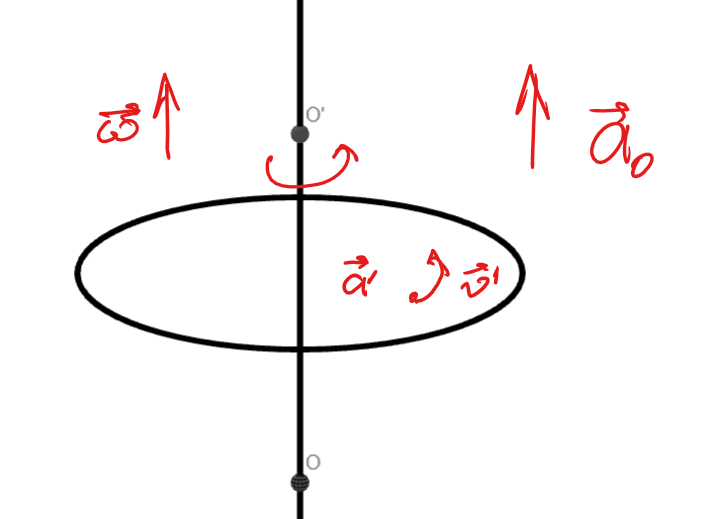
\includegraphics[height=5cm]{physics1/images/physics1_2024_09_30_1}
        \end{wrapfigure}

        Пусть $k$ - ИСО, $k^\prime$ - НИСО (неинерциальная СО), а $\vec{a}^\prime, \vec{v}^\prime$ - ускорение и скорость в системе $k^\prime$,
        а сама система $k^\prime$ движется с ускорением $\vec{a_0}$ и вокруг оси с угловой скоростью $|\vec{\omega}| = const$


        Тогда получаем ускорение в НИСО: $\vec{a}^\prime = \vec{a} + \omega^2 \vec{\rho} + 2 [\vec{v}^\prime \vec{\omega}] - \vec{a}_0$

        $\vec{a}$ - ускорение тела в системе $k^\prime$

        $\omega^2 \vec{\rho}$ - центробежное ускорение

    \end{minipage}

    \smallvspace

    $2 [\vec{v}^\prime \vec{\omega}]$ - ускорение Кориолиса

    $\vec{a}_0$ - поступательное ускорение (системы отсчета $k^\prime$ для $k$)

    $m\vec{a}^\prime = \underset{\sum \vec{F}}{\underbrace{m\vec{a}}} + \underset{\text{силы инерции (т. н. фиктивные)}}{\underbrace{m\omega^2 \vec{\rho} + 2m [\vec{v}^\prime \vec{\omega}] - m\vec{a}_0}}$ - основное уравнение динамики в НИСО

    $m \omega^2 \vec{\rho}$ - центробежная сила

    $2m [\vec{v}^\prime \vec{\omega}]$ - сила Кориолиса

    $m\vec{a}_0$ - поступательная сила инерции


    В НИСО возникают так называемые силы инерции (фиктивные), центробежная и Кориолиса связаны с вращением

    Сила Кориолиса будет действовать только на те тела, которые движутся

    Из закона всемирного тяготения можно вывести ускорение свободного падения гравитационное: $g_{\text{грав}} = G \frac{M_\text{З}}{R^2} = 9.81\dots9.83 \frac{\text{м}}{\text{с}^2}$

    Из этого получить ускорение эффективное: $g_\text{эфф} = g_\text{грав} + a_\text{цб} = 9.78\dots9.83$ (ускорение свободного падения уменьшается на 3 сотых из-за вращения)

    \subsection{Вес тела}

    \Def Вес тела - сила, с которой тело действует на неподвижную относительно него опору

    В случае опоры $|P| = |N|$ ($N$ - сила реакции опоры)

    Рассмотрим случай, когда тело находится в неподвижном состоянии на поверхности:

    $m\vec{g} + \vec{N} = 0 \quad\quad N - mg = 0 \quad\quad P = mg$

    Вес тела равен силе тяжести только при $\vec{a} = 0$ системы отсчета

    \subsection{Силы трения}

    Силы трения появляются при перемещении соприкасающихся тел или их частей относительно друг друга.
    Различают сухое и вязкое трение. К сухому трению относится трение покоя, трение скольжения и трение качения

    \textbf{Сила трения покоя} применима не телам, которые покоятся; она не может превышать некоторого максимального значения: $0 \leq F_\text{тр.} \leq \mu_0 N$ (где $\mu_0$ - коэффициент трения покоя)

    \textbf{Сила трения скольжения} возникает при движении соприкасающихся тел. В общем случае сила трения скольжения зависит
    от скорости движения, но для широкого класса тел равна максимальной силе трения покоя и подчиняется закону Амонтона-Кулона: $F_\text{тр} = \mu N$

    В задачах принимается, что $\mu_0 = \mu$, тогда во время покоя сила трения растет линейно, пока не достигнет $\mu N$, тогда тело начинает движение, и применяется сила трения скольжения

    \subsection{Как можно измерить массу тел?}

    Для измерения массы необходимо сравнить ее с другой, принятой за эталон. Сравним массы $m_1$ и $m_2$

    Опыт показывает, что в замкнутой системе - системе, в которой можно пренебречь взаимодействием с другими телами,
    выполняется соотношение:

    $\frac{\Delta \vec{v}_1}{\Delta \vec{v}_2} = \frac{m_2}{m_1}$

    $\Delta \vec{v}_1 \uparrow \downarrow \Delta \vec{v}_2 \quad\quad\quad v \ll c$

    $m_1 \Delta \vec{v}_1 = -m_2 \Delta \vec{v}_2$ или $m_1 \Delta \vec{v}_1 + m_2 \Delta \vec{v}_2 = 0$

    Импульс (количество движения) - векторная величина, равная произведению массы тела на его скорость: $\vec{p} = m\vec{v} \quad\quad [p] = \text{кг} \cdot \text{м/с}$

    Определение справедливо для материальной точки и для поступательного движения твердого тела

    Импульс системы материальных точек: $\vec{P} = \sum_{i = 1}^N \vec{p}_i$

    Для системы $N$ материальных точек ($\vec{F}_i$ - внешние силы)

    $\frac{d\vec{P}}{dt} = \sum \vec{F}_i \quad\quad\quad \vec{P} = const$

    Закон сохранения импульса - импульс замкнутой системы остается постоянным


    При изменении состояния системы всегда существуют такие величины, которые сохраняются с течением времени. Среди этих величин наиболее важное значение имеют импульс, энергия и момент импульса.

    Эти величины обладают свойством аддитивности – значение величин для системы, состоящей из частей, равно сумме значений для каждой из частей в отдельности.

    Законы сохранения – универсальные законы природы, связаны с фундаментальными свойствами пространства и времени.

    \begin{center}
        Закон сохранения импульса – однородность пространства

        Закон сохранения энергии – однородность времени

        Закон сохранения момента импульса – изотропность пространства
    \end{center}
    % end physics1_2024_09_30.tex



\end{document}

